\section{Reading data}
Although in the beginning it seemed as a simple task, reading the data
from the data-line turned out to be quite tricky. One would expect that
when the light sensor moves from a white region onto a black region,
it would result in a few readings of WHITE and then BLACK values. Instead
it results in WHITE - GREY - DARK GREY - BLACK values.

\subsection{Data encoding}
Because the light sensor is basically an analog input device, the outgoing
values have to be treated that way - as an analog signal. And as the device
is not that sensitive, we decided (for the sake of reliability) to reduce
the number of recognized colors to three: WHITE, GREY, BLACK.

This gives us the option to encode binary strings into a 3-level signal.
WHITE being the \textit{no-data}, \textit{synchronization} level and GREY
and BLACK being the \textit{data} levels, 0 and 1 respectively. Every
signal interval between two WHITE regions is considered to be one bit and
based on the maximal value (darkness of the color) we recognize its value.

This is a "peak value encoding" with automatic synchronization.
The encoding therefore delivers 1 bit of information for every two signal
elements (changes).

\begin{figure}[h]
\begin{center}
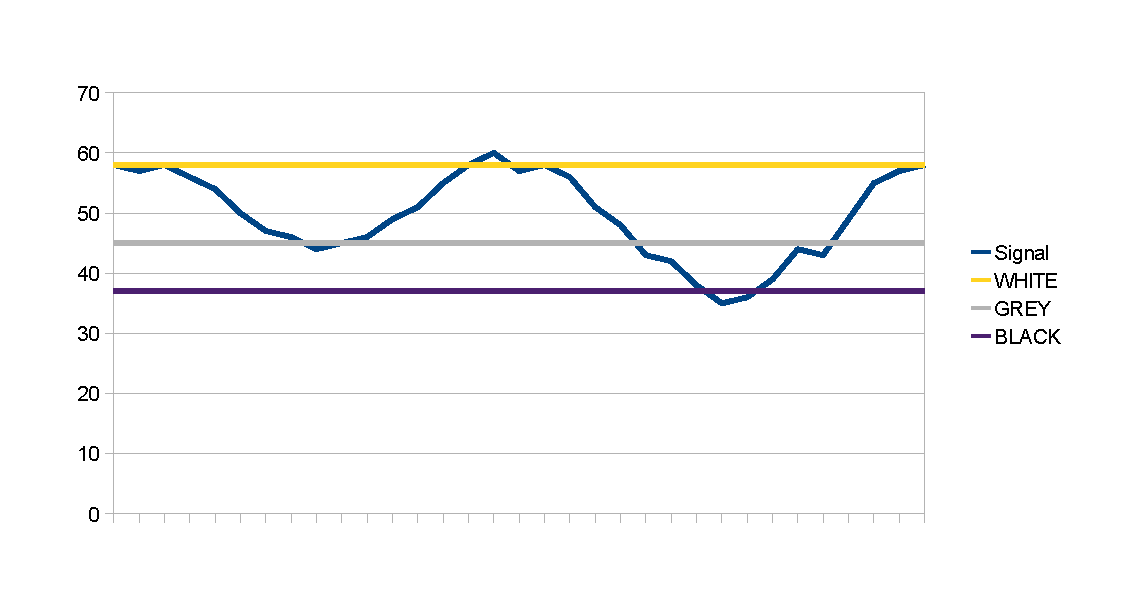
\includegraphics[width=0.75\linewidth]{light_signal.pdf}
\end{center}
\caption{Light sensor readings}
\end{figure}

\subsection{Various details}
After testing a few layouts and configurations we found that the best
results are achieved with \textit{data} stripes 2~cm thick and
\textit{synchronization} spaces about 3~cm thick. Thin stripes
tend to be overlooked by the robot, extra thick \textit{data} stripes
could be erroneously interpreted as multiple bits. Larger areas of white
do not matter much, although there is always the possibility of picking
up "noise" bits (e.g. dirt marks).

The cooperation of the line-following (main) and data-reading (slave) threads
proved to be essential. When the robot leaves the guiding line, it needs
to stop, adjust its direction and then continue again.
This often results in erroneously read or re-read bits, because the
data-line is not moving strictly in one direction. The master thread
therefore signals the slave thread when it is safe to read data values
(i.e. the robot is moving forward).

\subsection{Error handling}
To make the encoding as simple as possible, we implemented a
timeout-based reading termination to avoid control sequences in the data
flow. Every successfully read bit resets the timer, otherwise after
a specified timeout the reading process is terminated. This signals
the main line-following thread that it should terminate as well.

In the end the resulting array of bits is converted into an array of
2-bit \textit{bytes}. This implies an even number of bits, which is the
only error-checking performed by the decoder. Bit values are not checked
in any way as it would require more bits to be read.

